\documentclass{miniprojectreport}
\usepackage{miniprojectreportcommands}
\usepackage{lipsum}
\usepackage{graphicx}

\defstudentnameone{John Doe I}
\defstudentregnoone{1200XXXXX}

\defstudentnametwo{John Doe II}
\defstudentregnotwo{1200YYYYY}

\defstudentnamethree{John Doe III}
\defstudentregnothree{1200ZZZZZ}

\defprogramme{Computer Science and Engineering}

\defguide{John Doe}
\defguidedesignation{Senior Assistant Professor}
\defstudyduration{June 2019 - November 2019}

\title{Paper Title}
\date{18 November 2019}

\begin{document}
	\pagenumbering{roman}
	\makeminireportfirstpage
	\bonafide
	\acknowledgement{\lipsum[1]}
	\reportabstract{
		This is some dummy abstract. \lipsum[2]
	}{Random, Keywords, for, report}
	\newpage
	\tableofcontents
	\newpage
	\pagenumbering{arabic}
	\setcounter{page}{1}
	\chapter{Contents of the Base Paper}
		\setcounter{chapter}{1}
		\section{Paper Details}
		The details of the paper go here.
		\section{Introduction}
		\lipsum[3]
		\section{Proposed Solution}
		\lipsum[4]
		\subsection{The Dataset}
		\lipsum[5]
	\chapter{Mertis and Demerits of the Base Paper}
		\section{Existing Solution}
		\lipsum[6]
		\section{Merits}
		\lipsum[7]
		\section{Demerits}
		\lipsum[8]
	\chapter{Source Code}
	\section{Sample Class}
	Purpose of the sample class is to show a sample python syntax. To add more keywords or words to emphasize, add them to line 78 and 80 in the file named miniprojectreport.cls\\Also, this\cite{7457930} is a dummy citation.\\
\begin{python}
class SampleClass:
    def __init__(self):
        self.x = 10	
\end{python}
	
	\newpage
	\chapter{Snapshots}
	\section{Sample Output screens}
	Add Snapshots of your output screen like Figure \ref{fig1}.
	\begin{figure}
		\centering
		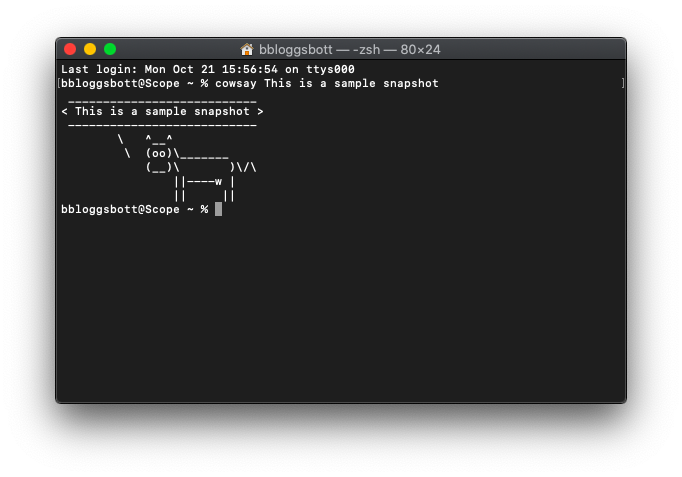
\includegraphics[width=\textwidth]{images/snapshot1}
		\caption{Sample Snapshot 1}
		\label{fig1}
	\end{figure}
	I'd suggest inverting color of terminal to save ink while printing like in Figure \ref{fig2}.
	\begin{figure}
		\centering
		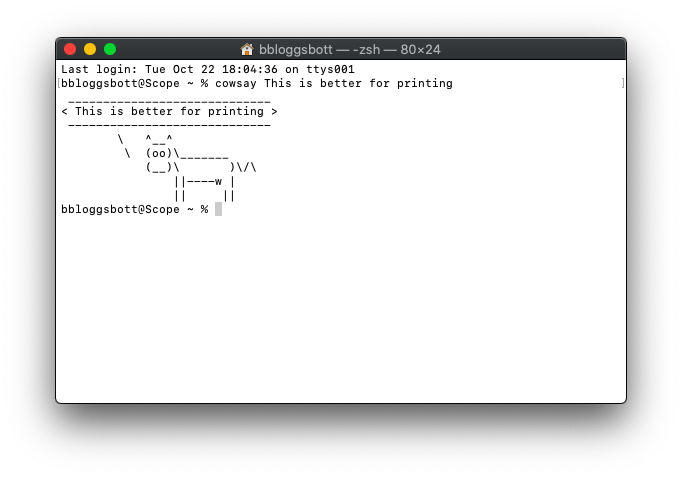
\includegraphics[width=\textwidth]{images/snapshot2}
		\caption{Sample Snapshot 2}
		\label{fig2}
	\end{figure}

	\chapter{Conclusion and Future Plans}
	\lipsum[9]\\

	\bibliography{miniprojectreportbib}
	
	\bibliographystyle{ieeetr}
	
\end{document}
